\chapter{Indirect communication}


\section{Introduction}

In [1] \emph{indirect communication} is defined as "communication between entities in a distributed system through an intermediary with no direct coupling between sender and receiver". Uncoupling may be established in two ways:

\begin{itemize}
	\item \textbf{Space} : The sender does not (need to) know the identity of the receiver.
	\item \textbf{Time} : The sender and receiver does not (need to) exist at the same time as the receiver.
\end{itemize}

\textbf{Table 1} categorizes a number of technologies according to their support for time and/or space uncoupling. Note the relationship between time uncoupling and asynchronous communication. However, in the case of strict uncoupling in time, the receiving end does not necessarily exist at the time of sending, as mentioned earlier [1].


\begin{table}
	\caption{Overview of space and time coupling for distributed communication paradigms.}
	\label{tab:}
	\begin{tabular}{p{100px} | p{125px} | p{125px}}
															& \textbf{Time-coupled} 	& \textbf{Time-uncoupled} \\
		\hline
		\textbf{Space-coupled} 		& Message-passing, RMI 		&  \\
		\textbf{Space-uncoupled} 	& IP multicast						& Publish-subscribe, tuple spaces, message queues \\
		\hline
	\end{tabular}
\end{table}

Typical applications of indirect communication is in mobile environments, cloud computing, and event dissemination where receivers are unknown or change rapidly [1].



\section{Paradigms}

\subsection{Group communication}

In group communication the messages within a distributed system are sent to a group, and from there sent to all other members of the group. The sender has no knowledge of the identities of the receivers, hence the indirection [1]. This kind of communication is called broadcasting where the sender forms a one-to-many relationship with the other members of the group.

Groups may be open or closed. In closed groups only members can multicast to it, opposed to open groups where processes outside the group can multicast to it as well.

\textbf{Figure 1} gives an overview of the basic operations of group management. The operation set for group communication is shown in \textbf{table 2}.


\begin{figure}
	\begin{center}
		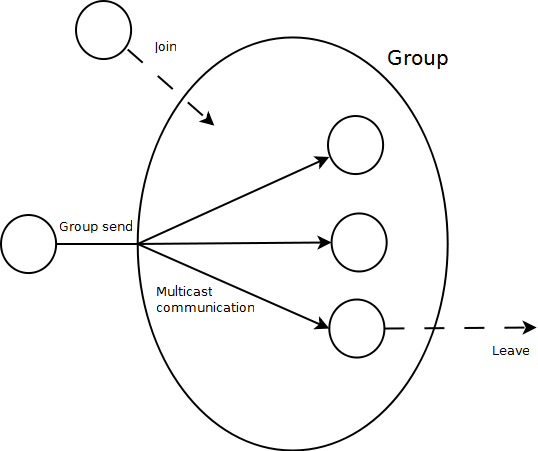
\includegraphics[width=0.5\textwidth]{img/groupcommunication}
	\end{center}
	\caption{Group membership management in group communication.}
	\label{fig:groupcommunication}
\end{figure}

\begin{table}
	\caption{Group communication API.}
	\label{tab:api:groupcommunication}
	\begin{tabular}{p{150px} | p{250px}}
		\textbf{Operation} & \textbf{Description} \\
		\hline
		join (group) & \emph{A process joins the group.} \\
		leave (group) & \emph{A process leaves the group.} \\
		send (group, message) & \emph{Send a message to the group. The group indirection layer propagates the message to all other members.} \\
		\hline
	\end{tabular}
\end{table}


\subsection{Publish-subscribe systems}

A publish-subscribe system is a platform where \emph{subscribers} can subscribe to certain events provides by \emph{publishers}. The system then matches published events against subscriptions. Subscribers then receive an update if successful matches are found.

Publishers form a one-to-many relationship with their subscribers, but the publishers do not know who is subscribed. Subscribers also do not need to know the publisher, as long as they can specify which kind of messages they would like to receive . Publish-subscribe systems are uncoupled in time as they provide asynchronous communication between senders and receivers [1].

The operations of a publish-subscribe system are listed in \textbf{Table 3}.


\begin{table}
	\caption{Publish-subscribe system API.}
	\label{tab:api:publishsubscribersystems}
	\begin{tabular}{p{150px} | p{250px}}
		\textbf{Operation} & \textbf{Description} \\
		\hline
		publish (event) 			& \emph{A publisher publishes an event.} \\
		subscribe (filter) 		& \emph{A subscriber subscribes to a set of events through a filter.} \\
		unsubscribe (filter) 	& \emph{A subscriber unsubscribes from a set of events.} \\
		notify (event) 				& \emph{Deliver events to its subscribers.} \\
	  advertise (filter) 		& \emph{A publisher declare the nature of the events they will produce.} \\
		unadvertise (filter) 	& \emph{A publisher revokes the advertisement.} \\
		\hline
	\end{tabular}
\end{table}



\begin{figure}
	\begin{center}
		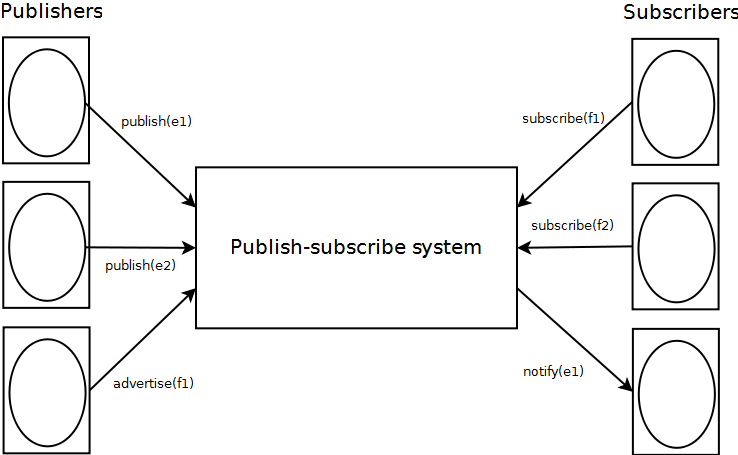
\includegraphics[width=0.6\textwidth]{img/publish-subscribesystem}
	\end{center}
	\caption{Publish-subscribe system architecture.}
	\label{fig:publish-subscribesystem}
\end{figure}




\subsection{Message queues}

Message queues are a form of message-oriented middleware. A message queue introduces a layer of indirection between \emph{producers} and \emph{consumers}. A producers sends messages to a queue, next consumers receive messages from these queues. Message queues are uncoupled in time, but not in space. The relation between a consumer and a producer through a message is one-to-one [1].

The operations that can be invoked on a message queue are listed in \textbf{table 4}.


\begin{table}
	\caption{Message queue API.}
	\label{tab:api:messagequeues}
	\begin{tabular}{p{150px} | p{250px}}
		\textbf{Operation} & \textbf{Description} \\
		\hline
		send (message) & \emph{A producer sends a message to the queue.} \\
		receive (message) & \emph{A blocking receive operation. The consumer will block until an appropriate message is available.} \\
		poll (message) & \emph{The consumer checks the status of the queue. A message is returned if available, else a negative signal.} \\
		notify (message) & \emph{Start listening for event notications if a message is available.} \\
		\hline
	\end{tabular}
\end{table}


Messages are usually added to the queue based on the first-in-first-out (FIFO) policy, but priorities may be used as well. Message queues try to ensure reliable delivery by persisting messages: messages are eventually delivered (time uncoupling). Messages are also only sent once and as received to provide integrity [1].

The consumers may receive messages by actively checking (polling) if messages are available, or by receiving notifications that messages have become available. Messages may be filtered based on certain properties [1].

\begin{figure}
	\begin{center}
		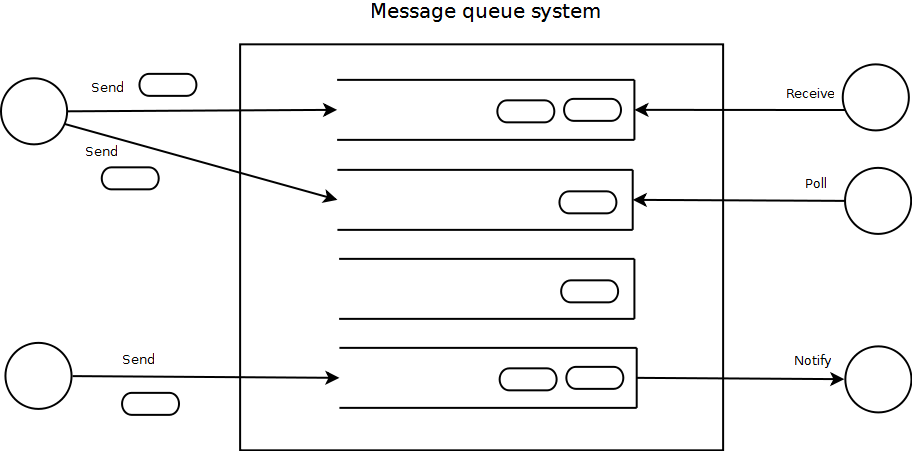
\includegraphics[width=0.7\textwidth]{img/messagequeues}
	\end{center}
	\caption{The message queue paradigm.}
	\label{fig:messagequeues}
\end{figure}



\subsection{Distributed shared memory}

The objective of distributed shared memory (DSM) is to share data between computers. Each computer has a local copy of the data. This data is kept up to date by passing messages between each node over the DSM middleware. \textbf{Table 5} shows the operations for DSM.

\begin{table}
	\caption{Distributed shared memory API.}
	\label{tab:api:dsm}
	\begin{tabular}{p{150px} | p{250px}}
		\textbf{Operation} & \textbf{Description} \\
		\hline
		read (data) 			& \emph{Read from the shared memory.} \\
		write (data) 			& \emph{Write to the shared memory} \\
		update (message) 	& \emph{Send an update message to the other members of the distributed shared memory.} \\
		\hline
	\end{tabular}
\end{table}


\begin{figure}
	\begin{center}
		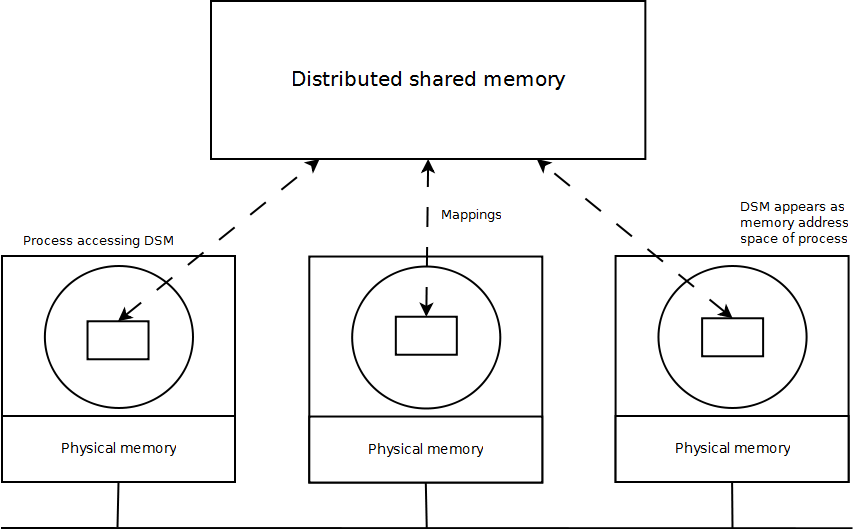
\includegraphics[width=0.6\textwidth]{img/dsm}
	\end{center}
	\caption{Distributed shared memory architecture.}
	\label{fig:dsm}
\end{figure}



\subsection{Tuple spaces}

A tuple space is a form of distributed memory where "processes communicate indirectly by placing tuples in a tuple space from which other processes can read and remove them" [1]. Space uncoupling is achieved as the sending and receiving processes may come from anywhere. Tuples may be taken from the space at any time and may even reside indefinately in the tuple space, thus achieving time uncoupling.

A tuple is typically of the form <var1, var2>, e.g. \emph{<"hugo",1.19>}. A number of operations can be executed on a tuple space as listed in \textbf{table 6}.


\begin{table}
	\caption{Tuple space API.}
	\label{tab:api:tuplespaces}
	\begin{tabular}{p{150px} | p{250px}}
		\textbf{Operation} & \textbf{Description} \\
		\hline
		read (tuple) 	& \emph{Reads a tuple from the tuple space.} \\
		take (tuple) 	& \emph{Extract a tuple from the tuple space.} \\
		write (tuple) & \emph{Write a new tuple to the tuple space.} \\
		\hline
	\end{tabular}
\end{table}


\begin{figure}
	\begin{center}
		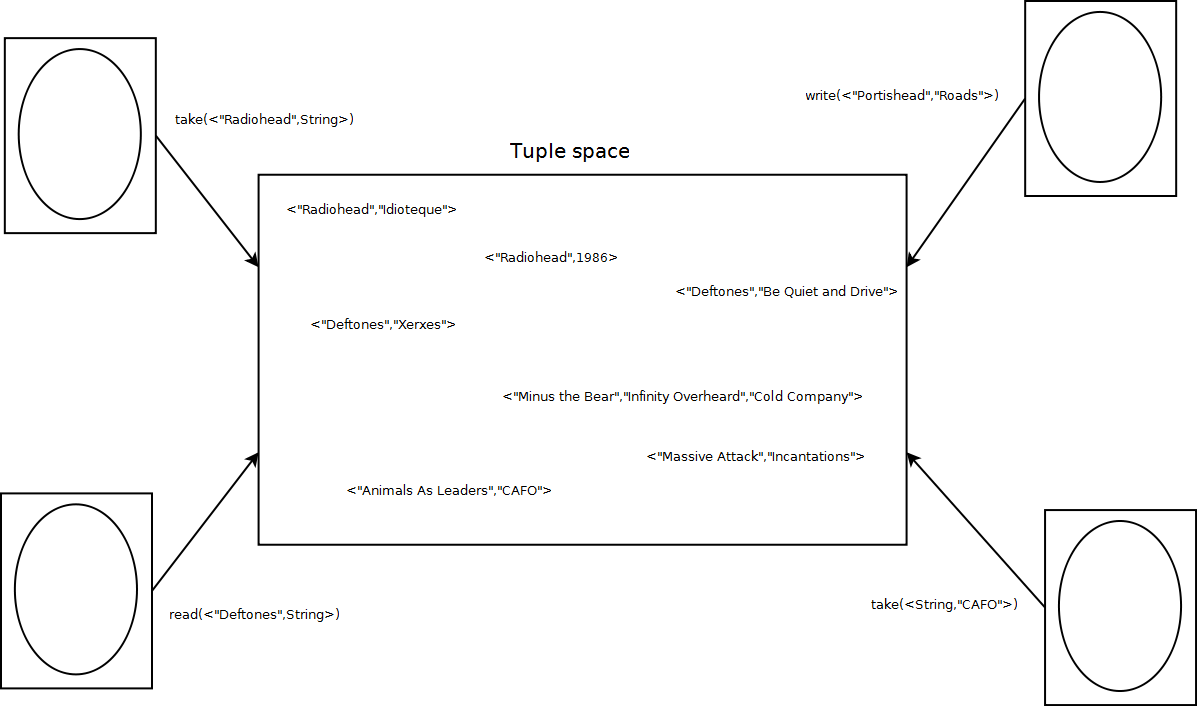
\includegraphics[width=0.6\textwidth]{img/tuplespace}
	\end{center}
	\caption{Tuple space abstract example.}
	\label{fig:tuplespace}
\end{figure}




\section*{References}

\begin{enumerate}[1]
	\item G. Coulouris, J. Dollimore, T. Kindberg and G. Blair, "Distributed Systems: Concepts and Design (5th Edition)", M. Horton, Red., Addison-Wesley, 2011, p. 1063.
\end{enumerate}